\documentclass[dvipdfmx, 11pt, aspectratio=169]{beamer}   % dvipdfmx で非 ASCII 画像も安全
\usetheme{metropolis}
\usecolortheme{metropolis}
\usepackage{booktabs}
\usepackage{tabularx}
\newcolumntype{L}{>{\raggedright\arraybackslash}X} % 左寄せの X 列
\usepackage{graphicx}
\usepackage{amsmath}
\usepackage{bm}
\usepackage{listings}
\usepackage{xcolor}
% コードのハイライト設定
\definecolor{codegreen}{rgb}{0,0.6,0}
\definecolor{codegray}{rgb}{0.5,0.5,0.5}
\definecolor{codepurple}{rgb}{0.58,0,0.82}
\definecolor{backcolour}{rgb}{0.95,0.95,0.92}

\lstdefinestyle{mystyle}{
    backgroundcolor=\color{backcolour},   
    commentstyle=\color{codegreen},
    keywordstyle=\color{blue},
    numberstyle=\tiny\color{codegray},
    stringstyle=\color{codepurple},
    basicstyle=\ttfamily\scriptsize,
    breakatwhitespace=false,         
    breaklines=true,                 
    captionpos=b,                    
    keepspaces=true,                 
    numbers=left,                    
    numbersep=5pt,                  
    showspaces=false,                
    showstringspaces=false,
    framexleftmargin=2em,
    showtabs=false,                  
    tabsize=2
}

\lstdefinelanguage{CUDA}{
  language=[ANSI]C++,                % C++ を継承
  morekeywords={
    __global__,__device__,__shared__,__constant__,__managed__,cudaError_t,
    __syncthreads,atomicAdd,atomicSub,atomicExch,dim3,blockIdx,threadIdx
  }
}

\lstdefinestyle{makefilestyle}{
  language        = make,        % listings 標準の make 言語
  basicstyle      = \ttfamily\footnotesize,
  keywordstyle    = \color{blue}\bfseries,
  commentstyle    = \color{codegreen},
  stringstyle     = \color{codepurple},
  numbers         = left,        % 行番号
  numberstyle     = \scriptsize\color{codegray},
  stepnumber      = 1,
  numbersep       = 6pt,
  tabsize         = 4,           % TAB=4 スペース
  showstringspaces= false,
  showtabs        = false,
  breaklines      = true,
  morekeywords    = {CC,CXX,LD,AR,CFLAGS,CXXFLAGS,LDFLAGS,RM,\%.o,all,clean}, % 独自キーワード
  xleftmargin     = 2em,         % コードブロック全体を右へ
  frame           = single,      % 枠線
  backgroundcolor = \color{backcolour}
}

\lstset{style=mystyle}
\title{CUDA: understand to be a genuine user}
\author{takigawa}
\institute{The university of Tokyo, EEIC, Taura Lab}
\date{\today}

%%%%%%%%%%%%%%%%%%%%%%%%%%%%%%%%%%%%%%%%
\begin{document}
%%%%%%%%%%%%%%%%%%%%%%%%%%%%%%
% タイトルスライド
\begin{frame}
  \titlepage       
\end{frame}
% 目次
\begin{frame}{Contents}
  \begin{enumerate}%[<+->]   % <+-> で 1 行ずつ出現
    \item What is CUDA?: Introduction
    \item A CUDA program for beginners
    \item How CUDA works
    \item Optimize CUDA program
    \item Practice Problems
  \end{enumerate}
\end{frame}
%%%%%%%%%%%%%%%%%%%%%%%%%%%%%%%
\section{What is CUDA?}
% 目次
\begin{frame}{Contents}
  \begin{enumerate}%[<+->]   % <+-> で 1 行ずつ出現
    \item What is CUDA?: Introduction
    \item \textcolor{gray}{A CUDA program for beginners}
    \item \textcolor{gray}{How CUDA works}
    \item \textcolor{gray}{Optimize CUDA program}
    \item \textcolor{gray}{Practice Problems}
  \end{enumerate}
\end{frame}
%%%%%
\begin{frame}{CUDA is the abstraction of GPU(s) for programmers}
  GPU (Graphical Processing Unit) is a device separated from CPU (Central PU).
  \begin{itemize}
    \item Code that runs on GPU must be designated as a kernel
    \item Data must be copied between CPU and GPU(s)
    \item A GPU is often called a \textcolor{blue}{\textit{"device"}}
    \item A CPU is often called a \textcolor{blue}{\textit{"host"}}
  \end{itemize}
  % figure
  \begin{columns}
    \column{0.45\textwidth}
    \begin{figure}
      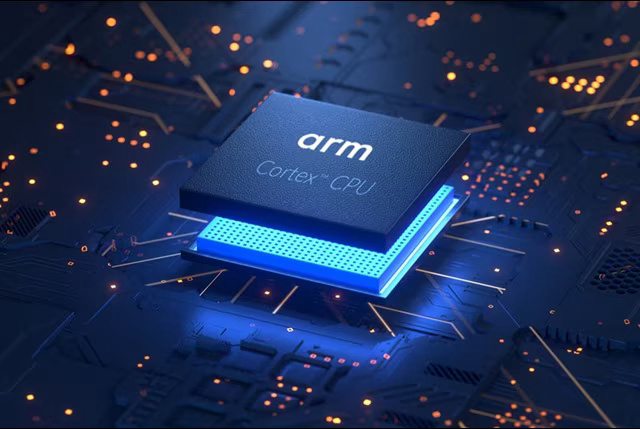
\includegraphics[scale=0.2]{img/host.png}
      \caption{Host}
    \end{figure}
    \column{0.55\textwidth}
    \begin{figure}
      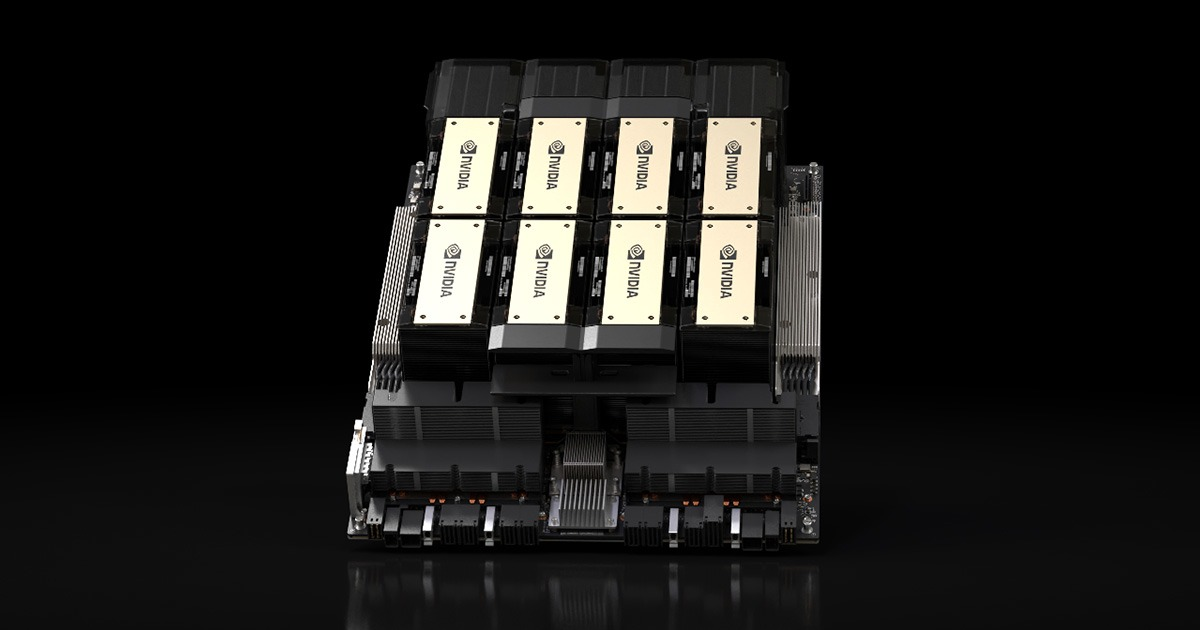
\includegraphics[scale=0.15]{img/device.jpg}
      \caption{Device}
    \end{figure}
  \end{columns}
\end{frame}
%%%%%%
\begin{frame}{CUDA is the abstraction of GPU(s) for programmers}
  CUDA is a platform for parallel computing on NVIDIA GPU.
  \begin{itemize}
    \item language extension: C/C++, Fortran
    \item tools: compiler(nvcc), debugger(cuda-gdb), profiler(Nsight Systems)
    \item APIs: Driver API, Runtime API
    \item Libraries: cuBLAS, cuFFT, cuDNN, etc.
  \end{itemize}
  Their common goal is to provide programmers with a "good" abstraction of GPU(s).
  How "good"?: usable, simple, highly affine to hardware(=easy to bring out the performance)
\end{frame}
%%%%%
\begin{frame}[fragile]{To compile/run CUDA programs: NVCC}
  \begin{block}{}
    \begin{lstlisting}
      nvcc -arch=sm_90 programs.cu%
\end{lstlisting}
  \end{block}
  \begin{itemize}
    \item compile with \lstinline|nvcc| command
    \item the natural extension of CUDA program is \lstinline|.cu|
    \item \lstinline|-arch| flag designates GPU Architecture
    \begin{itemize}
      \item \lstinline|compute_XX|: Virtual architecture
      \item \lstinline|sm_XX|: Physical architecture (SM generation)
    \end{itemize}
  \end{itemize}
\end{frame}
%%%%%%
\begin{frame}[fragile]{Interlude: How to know the proper architechture}
  Use \lstinline|cudaGetDeviceXXXXX| APIs and get device query.
  \begin{block}{\lstinline|device_query.cu|}
    \begin{lstlisting}[language=CUDA]
#include <cuda_runtime.h>
int deviceCount;
cudaError_t error = cudaGetDeviceCount(&deviceCount);
cudaDeviceProp deviceProp;
cudaGetDeviceProperties(&deviceProp, i);
      
printf("Device %d: %s\n", i, deviceProp.name);
printf("  Compute capability: %d.%d\n", deviceProp.major, deviceProp.minor);
printf("  Total global memory: %.2f GB\n", deviceProp.totalGlobalMem / (1024.0 * 1024.0 * 1024.0));
\end{lstlisting}
  \end{block}\vspace{-\baselineskip}
  or \vspace{-1.5\baselineskip}
  \begin{block}{}
    \begin{lstlisting}[language=bash]
  nvidia-smi --query-gpu=compute_cap
\end{lstlisting}
  \end{block}\vspace{-\baselineskip}
  The architecture for GH200 is \lstinline|sm_90|.
\end{frame}
%%%%%%%%%%%%%%%%%%%%%%%%%%%%%%%
\section{A CUDA program for beginners}
% 目次
\begin{frame}{Contents}
  \begin{enumerate}%[<+->]   % <+-> で 1 行ずつ出現
    \item \textcolor{gray}{What is CUDA?: Introduction}
    \item A CUDA program for beginners
    \begin{enumerate}
      \item Kernels; writing and launching
      % __global__ kernelFunction, kernelFunction<<nb, bs>>(arg1, arg2, ...)
      \item Host-Device Data Communication (+ Synchronization)
      % cudaMalloc, cudaMemcpy, cudaMallocManaged, cudaDeviceSynchronize
    \end{enumerate}
    \item \textcolor{gray}{How CUDA works}
    \item \textcolor{gray}{Optimize CUDA program}
    \item \textcolor{gray}{Practice Problems}
  \end{enumerate}
\end{frame}
%%%%%%%%%%
\subsection{Setting environment}
%%%%%
\begin{frame}[fragile]{Setting environment: Using GH200(s) on miyabi}
  \begin{enumerate}
    \item \url{https://miyabi-www.jcahpc.jp/login}にアクセスし、パスワード初期化を選択する
    \item 指示にしたがい、 Miyabi利用支援ポータルにアクセスする
    \item ドキュメント閲覧/Miyabiシステム利用手引書 をダウンロードする (Strongly recommended)
    \item 手引書のP.9 システム初回ログイン時の設定 の手順を完了する
    \item 手引書のP.22 SSHログイン/初回ログイン の手順を完了する (必ず緊急用スクラッチコードを控えること)
    \item (必要に応じて) エディタから2回目ログインを行う
  \end{enumerate}
  2要素認証が必須である。

  【注意】 ログインノード \lstinline|/home/cXXXXX|ではなく、計算ノード\lstinline|/work/gc64/cXXXXX|で作業する
\end{frame}
%%%%%%%%%%
\subsection{hello\_world}
%%%%%
\begin{frame}[fragile]{Sample program \#1: \texttt{hello\_world.cu}}
  See \url{https://github.com/gunnersgoestocl/cuda-introduction/tree/main/tutorial-legacy} for more information.
\begin{block}{}
  \begin{lstlisting}[language=CUDA]
#include <stdio.h>
#include <cuda_runtime.h>             // for Runtime APIs

__global__ void hello(){              // kernel function
    printf("Hello CUDA World !!\n");
}

int main() {
    hello<<< 2, 4 >>>();              // launch kernel
    cudaDeviceSynchronize();          // wait until kernel completes
    return 0;
}
  \end{lstlisting}
\end{block}
\end{frame}
%%%%%%
\begin{frame}[fragile]{3 files are required for execution on miyabi}
% .cu, makefile, .sh
  \begin{itemize}
    \item \lstinline|.cu| file: CUDA user program
    \item \lstinline|makefile|: compile and clean
    \item shell script: to submit batch job, see official docs for more info
  \end{itemize}
  \begin{columns}
    \column{0.5\textwidth}
    \begin{lstlisting}[style=makefilestyle, basicstyle=\ttfamily\tiny]
NVCC := nvcc
NVCCFLAGS := -arch=sm_90 -O3
# .cu ファイルから実行ファイルを生成
CUDA_EXECUTABLES := $(patsubst %.cu,%,$(wildcard *.cu))
# デフォルトのターゲット
all: $(C_EXECUTABLES) $(CUDA_EXECUTABLES)
# .cu ファイルから実行ファイルを生成
%: %.cu
	$(NVCC) $(NVCCFLAGS) $< -o $@
# clean ターゲットの定義
.PHONY: clean
clean:
	rm -f $(CUDA_EXECUTABLES)
\end{lstlisting}
    \column{0.5\textwidth}
    \begin{lstlisting}[language=sh]
#!/bin/bash
#PBS -q debug-g
#PBS -l select=1
#PBS -W group_list=gc64
#PBS -j oe

module purge
module load cuda

cd ${PBS_O_WORKDIR}
./a.out 256
\end{lstlisting}
  \end{columns}
\end{frame}
%%%%%%
\begin{frame}[fragile]{Contents of .cu file: kernel function}
% keywords (__global__ etc.)
  \begin{itemize}
    \item \textcolor{blue}{"kernel"} (sometimes \textcolor{blue}{"GPU kernel"}): A function that runs on GPU
    \begin{itemize}
      \item SYNTAX: An ordinary C/C++ function that returns nothing (\lstinline|void|)
      \item SYNTAX: Add \textcolor{blue}{\lstinline|__global__|} keyword beforehand
    \end{itemize}
  \end{itemize}
  \begin{block}{}
    \begin{lstlisting}[caption=kernel template, language=CUDA]
__global__ void f(...args...) { ...body... }
    \end{lstlisting}
  \end{block}
\end{frame}
%%%%%%
\begin{frame}[fragile]{Contents of .cu file: launching kernel by a host}
% specify the number of threads (and blocks), you can use dim3 struct
  A host (CPU) launches a kernel to devices.
  \begin{itemize}
    \item Programmers must specify the number of threads by \lstinline|<<nb, bs>>|
    \begin{itemize}
      \item \lstinline|nb|: Number of Blocks (per grid) (sometimes \lstinline|gridDim|)
      \item \lstinline|bs|: Block Size (sometimes \lstinline|blockDim|)
    \end{itemize}
    \item \lstinline|nb * bs| is the number of CUDA threads created
  \end{itemize}\vspace{-1.5\baselineskip}
  \begin{block}{}
    \begin{lstlisting}[language=CUDA]
      // ... code run on host ...
      
      f<<gridDim, blockDim>>(...args...);
\end{lstlisting}
  \end{block}\vspace{-\baselineskip}
  \begin{itemize}
    \item \lstinline|nb, bs| can be ${1,2,3}$-Dimensional using type \lstinline|dim3|
  \end{itemize}\vspace{-1.5\baselineskip}
  \begin{block}{}
    \begin{lstlisting}[language=CUDA]
    dim3 block(x_threads_block, y_threads_block);    // x, y(, z)
    dim3 grid(x_blocks_grid, z_blocks_grid);         // x, y(, z)
          
    f<<grid, block>>(...args...);
\end{lstlisting}
  \end{block}
\end{frame}
%%%%%%
\begin{frame}[fragile]{Interlude: register values programs can explicitly use}
% gridDim, blockIdx, blockDim, threadIdx
\begin{itemize}
  \item Threads which executes a single instruction can be executed in parallel.
  \item So, programmers are expected to make the kernel visible to all threads as the same instruction.
  \item For this perspective, a unique ID of each thread (= the loop index) is the key.
\end{itemize}
In CUDA, each kernel can access its own thread ID through built-in variables on the \href{https://docs.nvidia.com/cuda/parallel-thread-execution/#special-registers}{Special Registers}.
\begin{itemize}
  \item \lstinline|blockDim.{x,y} = bs| (the block size)
  \item \lstinline|gridDim.{x,y} = nb| (the number of blocks)
  \item \lstinline|threadIdx.{x,y} = | the thread ID within a block $(\in [0, bs))$
  \item \lstinline|blockIdx.{x,y} = | the thread's block ID $(\in [0, nb))$
  \item[->] \lstinline|blockDim.x * blockIdx.x + threadIdx.x| could be the loop index
\end{itemize}
\end{frame}
%%%%%%%%
\subsection{hello\_gpu}
%%%%%
\begin{frame}[fragile]{Sample program \#2: \texttt{hello\_gpu.cu}}
\begin{block}{}\vspace{-\baselineskip}
  \begin{lstlisting}[language=CUDA, basicstyle=\ttfamily\tiny]
#include <stdio.h>
#include <cuda_runtime.h>

__device__ void gpuAdd(int *number){  *number += 1; }
__global__ void callGpu(int *number){  gpuAdd(number); }

int main(){
  int device_id = 0;  cudaSetDevice(device_id); //device set up
  int *a = (int*)malloc(sizeof(int));  *a = 0;  //allocate memory on host(cpu)
  int *a_dev = 0;  cudaMalloc((void**)&a_dev, sizeof(int)); // allocate memory on gpu
  cudaMemcpy(a_dev, a, sizeof(int), cudaMemcpyHostToDevice);  // memcpy host -> device
  // execute
  callGpu<<<1, 1>>>(a_dev);
  cudaDeviceSynchronize(); // Wait until GPU processing finishs.
  
  cudaMemcpy(a, a_dev, sizeof(int), cudaMemcpyDeviceToHost);  // memcpy device -> host 
  cudaFree(a_dev);  // free

  printf("ans: %d \n", *g); return 0; // display the answer
}
\end{lstlisting}
\end{block}
\end{frame}
%%%%%
\begin{frame}{Data communication between H \& Ds: overview}
% cudaMalloc, cudaMemcpy
  \begin{itemize}
    \item Host memory and device memory are (basically) \textcolor{red}{\textit{separete}}
    \item The device(D) cannot access data on the host(H) and vice versa by hardware
    \begin{itemize}
      \item Access to another memory (including that of another device) causes \lstinline|Segfault|
    \end{itemize}
    \item Software need to explicitly specify when and what to communicate between H \& D
  \end{itemize}
\end{frame}
%%%%%
\begin{frame}[fragile]{Data communication between H \& Ds: template to send}
  \begin{enumerate}[<+->]
    \item allocate data of the same size both on host and device
\begin{lstlisting}[language=CUDA]
size_t sz = sizeof(int)*len;
int *a = (int*)malloc(sz);
int *a_dev = 0;  cudaMalloc((void**)&a_dev, sz);
// (void**)&a_dev is the address of the pointer variable (a_dev)
// Head address of GPU global memory is written to a_dev
\end{lstlisting}
    \item the host works on the kinda initialization of the host data
\begin{lstlisting} [language=C]
for ( ... ) { a[i] = ... } // on host, initialize input data of kernel
\end{lstlisting}
    \item copy the data to the device
\begin{lstlisting} [language=CUDA]
cudaMemcpy(a_dev, a, sz, cudaMemcpyHostToDevice); // target address, source address, size, keyword
\end{lstlisting}
    \item pass the device pointer to the kernel
\begin{lstlisting}[language=CUDA]
f<<nb, bs>>(a_dev, ...);
\end{lstlisting}
    \end{enumerate}
\end{frame}
%%%%%
\begin{frame}[fragile]{Data communication between H \& Ds: template to retrieve}
  \begin{enumerate}[<+->]
    \item allocate data of the same size both on host and device
\begin{lstlisting}[language=CUDA]
size_t sz = sizeof(int)*len;
int *r = (int*)malloc(sz);                        // host memory
int *r_dev = 0;  cudaMalloc((void**)&r_dev, sz);  // device memory
\end{lstlisting}
    \item pass the device pointer of receptacle to the kernel
\begin{lstlisting}[language=CUDA]
f<<nb, bs>>(...,r_dev, ...);  // args must include pointer(s) of input and output
\end{lstlisting}
    \item copy the data to the device
\begin{lstlisting} [language=CUDA]
cudaMemcpy(r, r_dev, sz, cudaMemcpyDeviceToHost); // target address, source address, size, keyword
\end{lstlisting}
    \end{enumerate}
\end{frame}
%%%%%
\begin{frame}[fragile]{Host-Device synchronization}
  \begin{itemize}
    \item A kernel call and the host overlap.
    \item Multiple kernel calls are serialized on the GPU side, by default (Host basically cannot control)
    \begin{itemize}
      \item \textcolor{blue}{Grid} is an abstraction of a one time launch of the kernel.
      \item Grid is managed using a data struct FIFO queue called \textcolor{blue}{Stream}
      \item If you want to execute multiple kernel calls concurrently, you must use multiple Streams or Devices.
    \end{itemize}
    \item \lstinline|cudaDeviceSynchronize()| is an API to wait for the kernel to finish
  \end{itemize}
  \begin{columns}
    \column{0.4\textwidth}
    \begin{lstlisting}
h0();
g0<<...,...>>();
h1();
g1<<...,...>>();
cudaDeviceSynchronize();
h2();
\end{lstlisting}
    \column{0.6\textwidth}
    \begin{itemize}
      \item \lstinline|g0| might overlap with \lstinline|h1|
      \item \lstinline|g0| and \lstinline|g1| do not overlap because they are assigned to the same stream 0
      \item \lstinline|h2|s does not overlap with anything because of \lstinline|cudaDeviceSynchronize()|
    \end{itemize}
  \end{columns}
\end{frame}
%%%%%%%%
\begin{frame}{(+) "Programmer-free" data communication between H \& Ds}
% cudaMallocManaged, Unified Memory
  \begin{itemize}[<+->]
    \item Recent NVIDIA GPUs support \textcolor{blue}{Unified Memory} that \textbf{eliminate} the need for 
    \begin{itemize}
      \item explicit data movement between host and device memory
      \item dual pointer management
    \end{itemize}
    \item \textcolor{blue}{cudaMallocManaged} is an API that hides the copy of data between the host and devices
    \begin{itemize}
      \item The CPU and GPU page tables are linked at the unified virtual address, and a hardware page fault fires the moment a GPU/CPU accesses a page.
      \item The moment a GPU/CPU accesses a page, a hardware page fault fires and the page is moved on-demand.
      \item Coherency is ensured at the kernel synchronization point.
    \end{itemize}
  \end{itemize}
  Sample Code: \texttt{vecadd}
\end{frame}
%%%%%
\begin{frame}[fragile]{Conventional vs Unified Memory}
  \begin{table}
    \centering
    {\footnotesize
      \begin{tabularx}{\textwidth}{@{}l L L@{}}
        Purpose & Conventional (\lstinline|cudaMalloc|+\lstinline|cudaMemcpy|) & Unified Memory (\lstinline|cudaMallocManaged|)\\\midrule[1pt]
        Memory Management & allocates \textbf{separate buffers} for host and device, and makes copy explicit & \textbf{single pointer} can be referenced from either CPU/GPU\\\midrule
        copy & All buffer transfers each time \lstinline|cudaMemcpy()| is called & \textbf{automatic transfer per page} (on demand) \\\midrule
        address space & different values for CPU and GPU & \textbf{Unified Virtual Address (UVA)}-share same value \\\midrule
        oversubscribe & impossible & GPU Can allocate more than the memory capacity and swap unused pages to the host \\\midrule
        Optimization API & None & Manual tuning of placement with \lstinline|cudaMemPrefetchAsync|, \lstinline|cudaMemAdvise|\\
        \bottomrule
      \end{tabularx}
    }
  \end{table}
\end{frame}
%%%%%
% \begin{frame}{What happens behind \texttt{cudaMallocManaged}?}
%   \begin{columns}[T]
%     \begin{column}{0.47\textwidth}
%       \begin{enumerate}[<+->, series=cudaMallocManaged]
%         \item Allocation
        
%         Driver 
%         \item
%       \end{enumerate}
%     \end{column}
%     \column{0.01\textwidth}
%     \centering\vrule width 0.4pt
%     \begin{column}{0.47\textwidth}
%       \begin{enumerate}[<+->, series=cudaMallocManaged, resume]
%         \item 
%       \end{enumerate}
%     \end{column}
% \end{frame}
%%%%%%%%%%%%%%%%%%%%%%%%%%%%%%%
\section{HOW CUDA works}
% 目次
\begin{frame}{Contents}
  \begin{enumerate}%[<+->]   % <+-> で 1 行ずつ出現
    \item \textcolor{gray}{What is CUDA?: Introduction}
    \item \textcolor{gray}{A CUDA program for beginners}
    \item How CUDA works
    \begin{enumerate}
      \item Architecture of NVIDIA GPU
      % GPU unit, global memory, stream processor
      \item Grid, block, thread; abstractions by CUDA
      % block-SM, grid-GPU unit
      \item Warp; Parallel Thread eXecution
      % warp consists of 32 threads, SIMD, why threadIdx/blockIdx
      \item Stream: beyond Grid
      % stream is a FIFO queue, stream ID
      \item Memory Hierarchy in CUDA
      % global memory, shared memory, cache
      \item Resolving race condition on CUDA
      % atomicAdd, barrier synchronization, reduction(, cooperative groups)
    \end{enumerate}
    \item \textcolor{gray}{Optimize CUDA program}
    \item \textcolor{gray}{Practice Problems}
  \end{enumerate}
\end{frame}
%%%%%%%%%
\subsection{Architecture of NVIDIA GPU}
\begin{frame}{Architecture of NVIDIA GPU: GPU unit}
% global memory, SM, link etc.
\vspace{-\baselineskip}
\begin{columns}
  \column{0.45\textwidth}
  \begin{figure}
    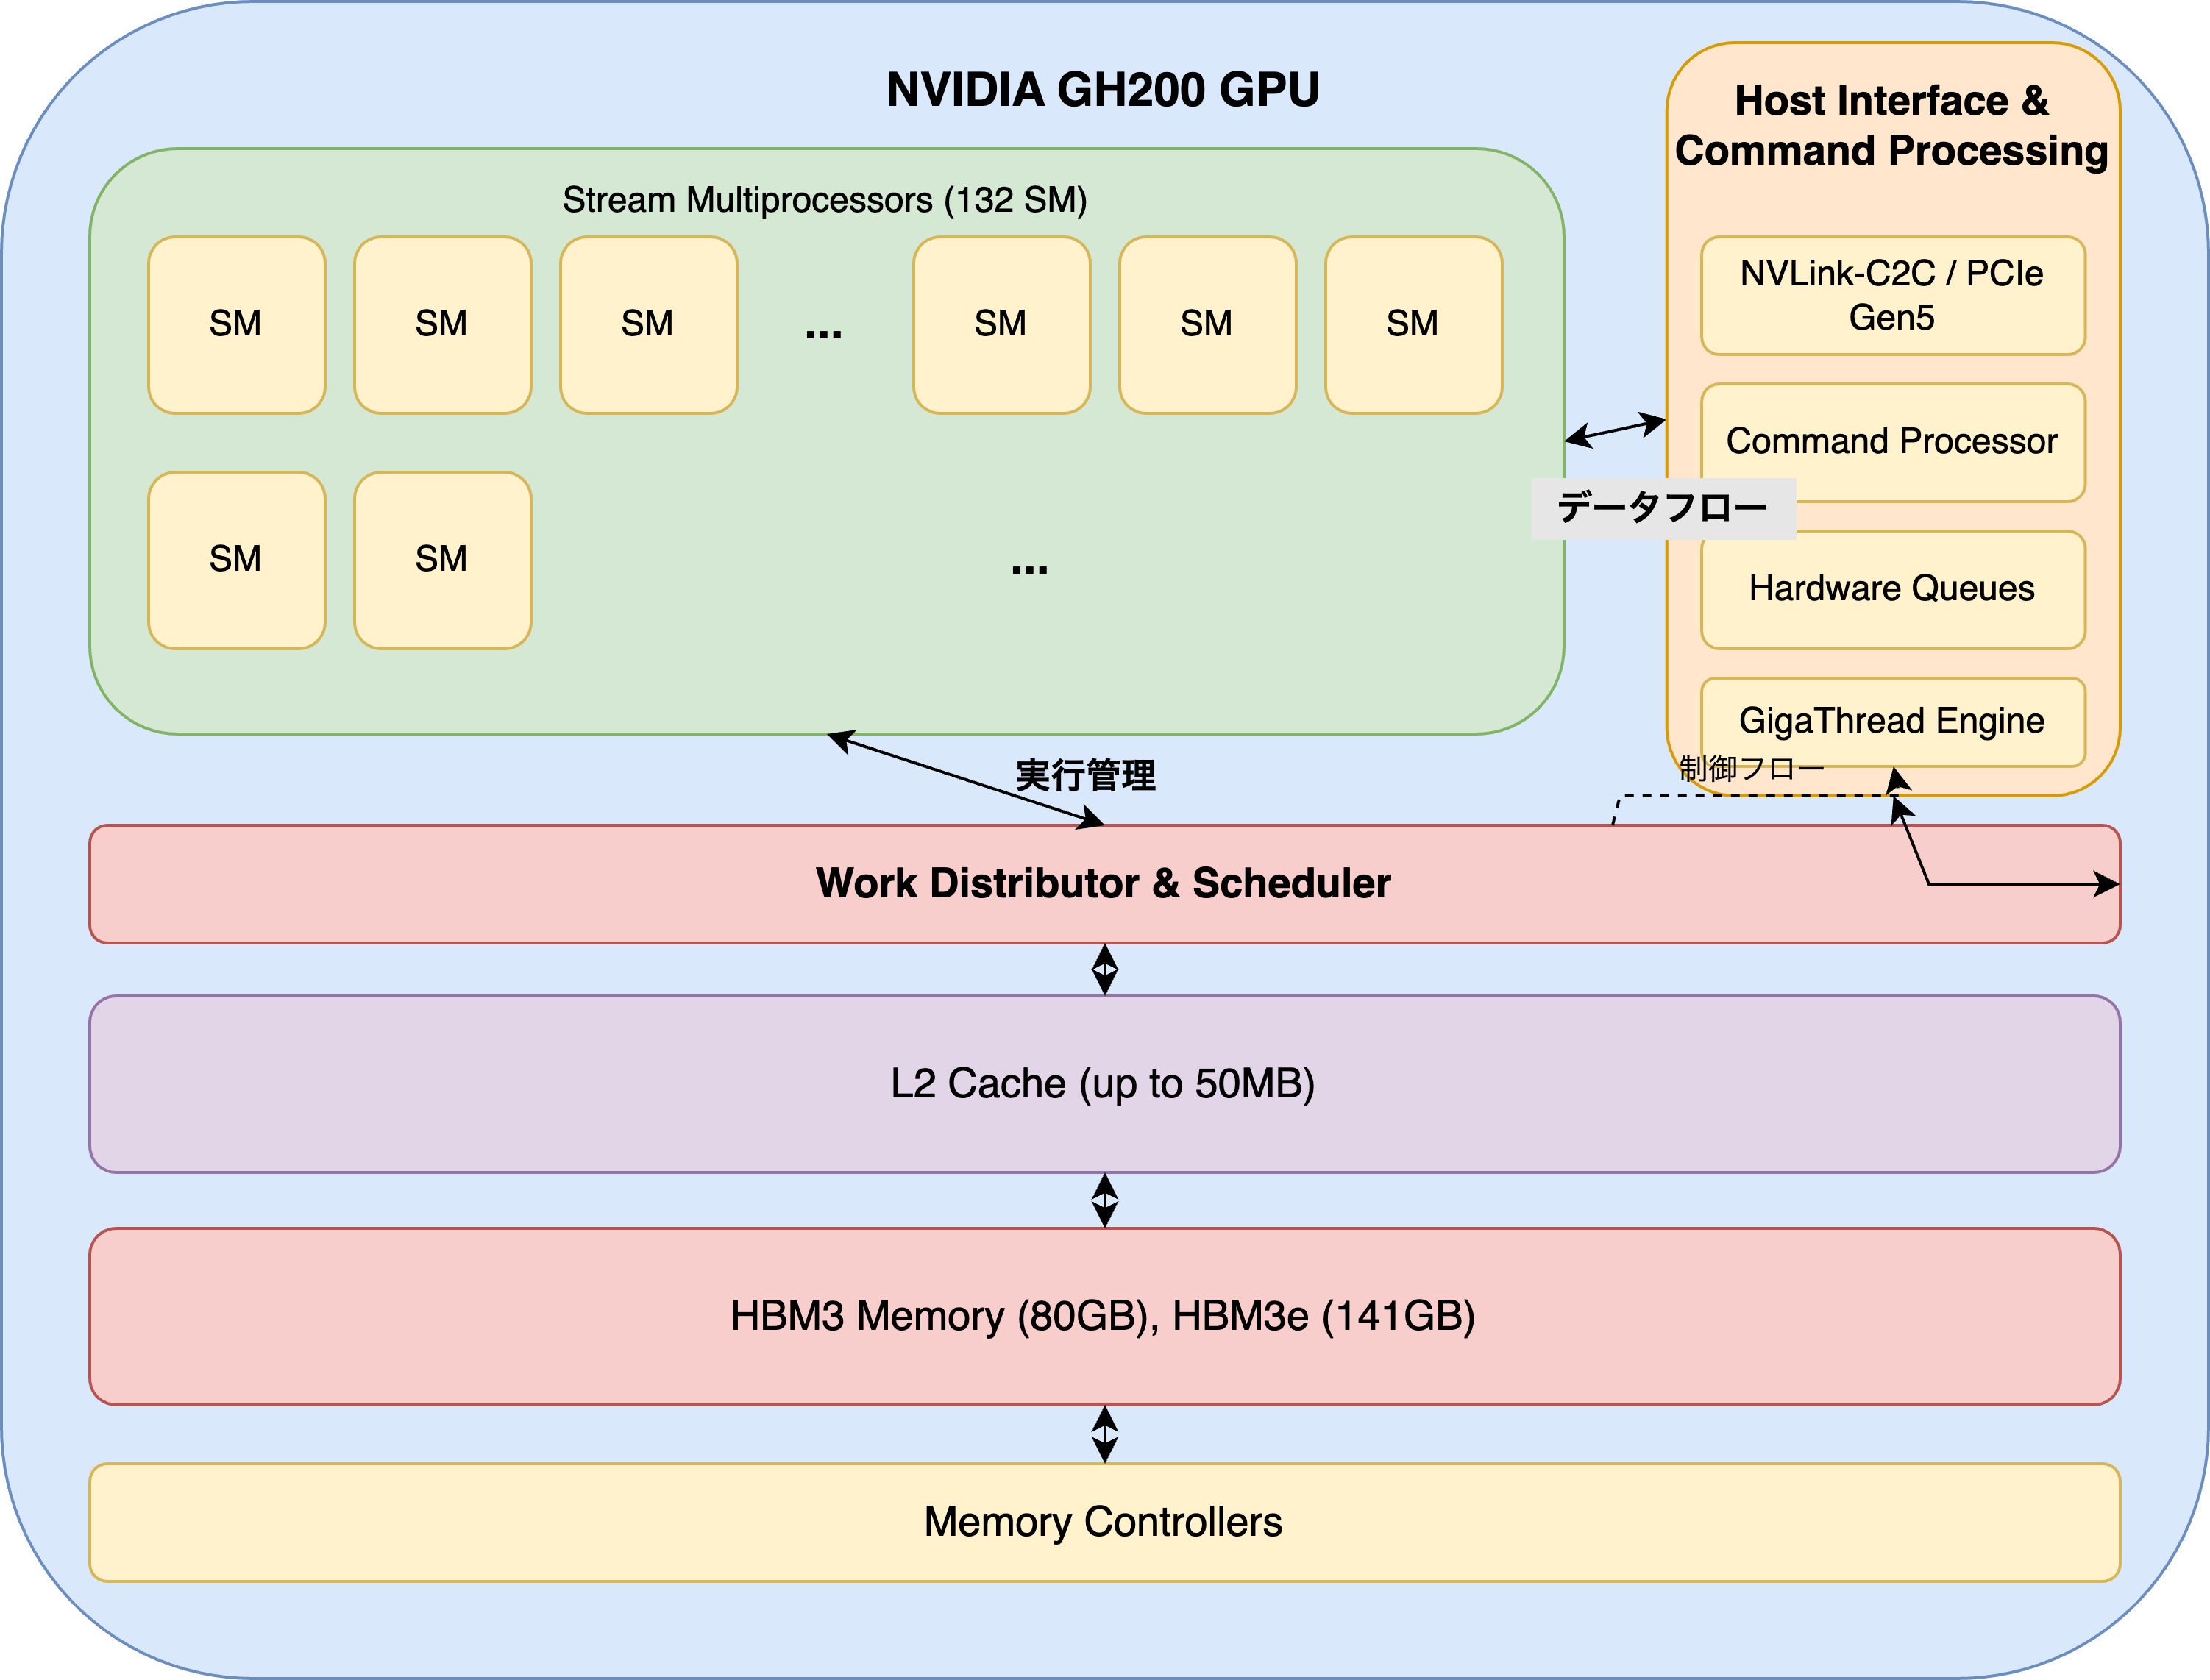
\includegraphics[scale=0.28]{img/gpuUnit.png}
    \caption{Device GPU}
  \end{figure}
  \column{0.49\textwidth}
  {\footnotesize
  \begin{itemize}
    \item GBM3 Memory
    
    known as \textcolor{blue}{global memory}, which has large capacity but slow access speed
    \item \textcolor{blue}{Stream Multiprocessor (SM)}
    
    In charge of multiple blocks, performs the operations that make up the kernel in parallel.
    \item Host Interface \& Command Processing

    Interface to communicate with the host CPU, and a command processing unit that manages the execution of commands.
  \end{itemize}
  }
\end{columns}
\end{frame}
%%%%%
\begin{frame}{Architecture of NVIDIA GPU: Stream Multiprocessors}
% CUDA core, regfile, Warp scheduler
\vspace{-\baselineskip}
\begin{columns}
  \column{0.47\textwidth}
  \vspace{\baselineskip}
  \begin{figure}
    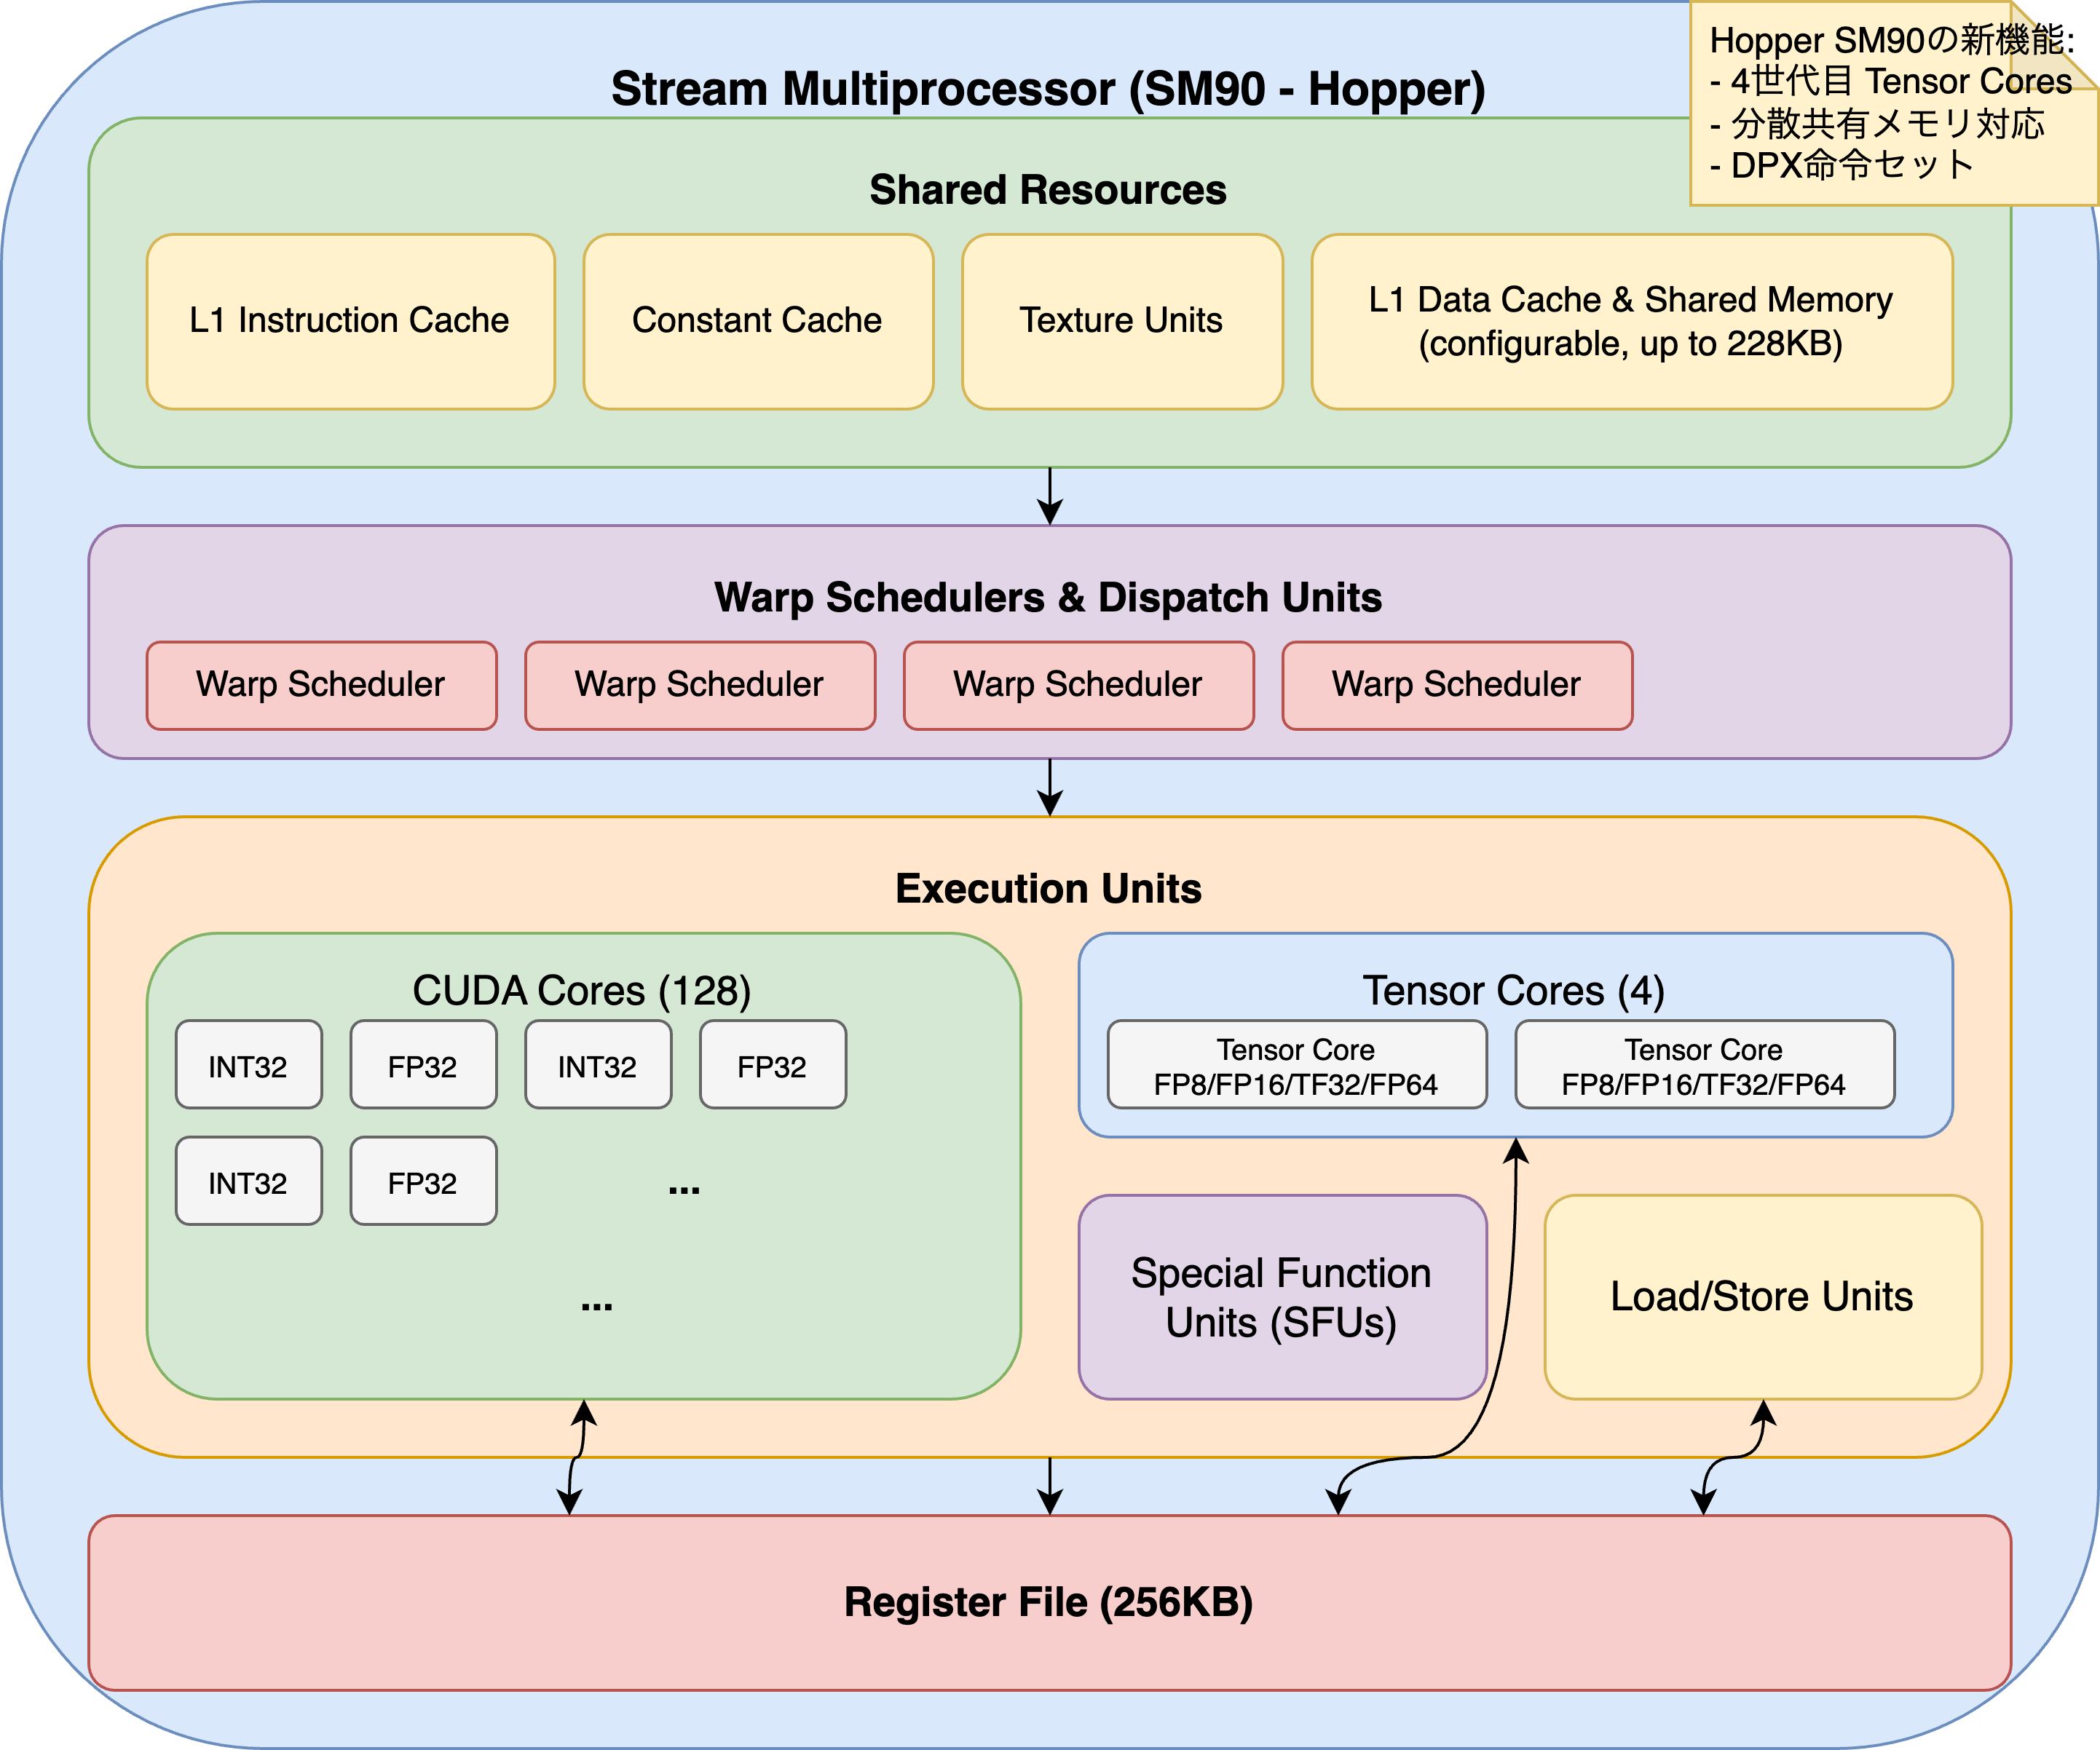
\includegraphics[scale=0.28]{img/sm90.png}
    \caption{Device GPU}
  \end{figure}
  \column{0.47\textwidth}
  {\footnotesize
  \begin{itemize}
    \item \textcolor{blue}{shared memory}
    
    has small capacity but relatively fast access speed
    \item \textcolor{blue}{Warp scheduler}

    Manage parallel execution on CUDA cores in units of Warps that comprise blocks allocated to the SM
    \item \textcolor{blue}{CUDA core}: The core that performs the actual computation
    \item \textcolor{blue}{Tensor core}: The core specialized for matrix operations
  \end{itemize}
  }
\end{columns}
\end{frame}
% %%%%%
% \begin{frame}{Architecture of NVIDIA GPU: Stream Multiprocessors}
% % cache, shared memory

% \end{frame}
%%%%%%%%
\subsection{Grid, block, thread; abstractions by CUDA}
%%%%%
\begin{frame}{3 easy pieces about hardware - software}
Programmers know 3 things about CUDA: Grid, Block, Thread
  \begin{itemize}
    \item (Review) \textcolor{blue}{Grid} corresponds to a one time launch of the kernel.
    \begin{itemize}
      \item A \textcolor{blue}{Grid} is assigned to a single GPU unit (i.e., a single device)
      \item (Review) \textcolor{blue}{Grid} is a collection of \textcolor{blue}{Blocks}
    \end{itemize}
    \item A \textcolor{blue}{Block} is the unit of dispatching to an SM
    \begin{itemize}
      \item A \textcolor{blue}{Block} is assigned to a single SM 
      
      i.e., once a block starts running, it stays on the SM (= occupies registers and shared memory) all the way until it finishes
      \item (Review) A \textcolor{blue}{Block} is a collection of \textcolor{blue}{Threads}
    \end{itemize}
    \item A \textcolor{blue}{Thread} is the smallest unit of execution
    \item A \textcolor{blue}{Thread} is assigned to a single CUDA core
  \end{itemize}
\end{frame}
%%%%%
\begin{frame}{Motivation: You may have questions like ...}
% 3 key questions to understand CUDA abstraction
  \begin{enumerate}
    \item Is it allowed for a \lstinline|block| to have \textcolor{red}{more \lstinline|thread|s than the number of \textbf{processors(CUDA cores)}} in the allocated \textbf{SM}, and if so, how is this handled?
    \item Is it allowed to have \textcolor{red}{more \lstinline|block|s than the number of \textbf{SM}s} that make up the \textbf{GPU unit} corresponding to the \lstinline|grid|, and if so, how is this handled?
    \item How is the execution across \textcolor{red}{multiple \lstinline|grid|s} handled?
  \end{enumerate}
  Hints:
  \begin{itemize}
    \item \lstinline|thread|s belonging to the same \lstinline|block| are executed by the same \textbf{SM}, this does \textcolor{red}{NOT} mean they are executed in parallel. 
    \item A \textbf{SM} is assigned to a \lstinline|block|, but this does \textcolor{red}{NOT} mean that an \textbf{SM} can only be in charge of one \lstinline|block|.
  \end{itemize}
\end{frame}
%%%%%%%%
\subsection{Warp: Parallel Thread eXecution}
%%%%%
\begin{frame}{Warp: The way to realize "Parallel" Thread eXecution}
 % Parallelism in your program is sometimes helped by Concurrency
  \begin{itemize}
    \item The unit of \textcolor{blue}{instruction execution} in the SM is a \textcolor{blue}{\textbf{Warp}}
    \item The number of threads that make up a warp has always been \textbf{32}.
    \item Each thread in a warp shares an instruction pointer (i.e, executes the same instruction at the same time).
    \item The warp scheduler selects a warp from the ready queue (Warp pool) and executes the instruction.
  \end{itemize}
\end{frame}
%%%%%
\begin{frame}{Hierarchy within an SM}
  % thread < warp < block < SM
  Parallelism within an Stream Multiprocessor consists of three levels.

  \textcolor{blue}{
  thread $\subset$ warp $\subset$ block $\subset$ SM 
  }
  \begin{columns}
    \column{0.60\textwidth}
    \begin{figure}
      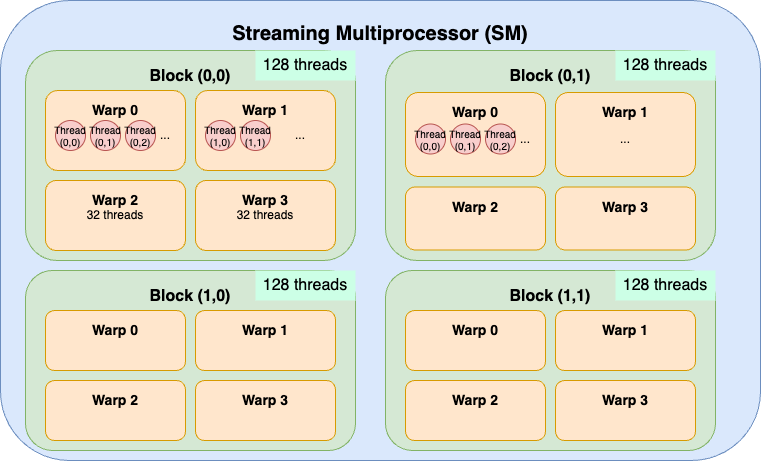
\includegraphics[scale=0.3]{img/smHierarchy.png}
    \end{figure}
    \column{0.45\textwidth}
    \begin{itemize}
      \item (recap) A group of \textcolor{blue}{$32$} CUDA threads makes a \textcolor{blue}{warp}
      \item A group of \textcolor{blue}{$bs/32$} warps makes a \textcolor{blue}{block}
      \item There are multiple blocks active on a single SM
    \end{itemize}
  \end{columns}
\end{frame}
%%%%%
\begin{frame}{Limitation of Hardware: performance degradation}

\end{frame}
%%%%%%%%
\subsection{Stream: beyond Grid} % How is the execution across \textcolor{red}{multiple \lstinline|grid|s} handled?
%%%%%%
\begin{frame}{Stream}
  (review) As long as multiple kernels are submitted to the same stream(i.e., the default stream), 
  they are always executed in series on the GPU side.

  $\because$ If program doesn't specify Stream when launching a kernel, the grid is automatically assigned to \textcolor{blue}{legacy stream 0}.
  \begin{itemize}
    \item \textcolor{blue}{Stream} is a \textbf{FIFO queue} that binds the sequence of operations passed by the host to the GPU.
  \begin{quote}
    \vspace{0.2\baselineskip}
    \small
    The host runtime writes the operation to the command buffer and queues up entries with the same \textcolor{blue}{stream ID}
    ; the GPU grabs the queue on \textcolor{purple}{doorbell notification} and distributes it to the hardware engine (Device), keeping each stream in order.
  \end{quote}\vspace{-\baselineskip}
  \begin{itemize}
    \item \textcolor{blue}{Grid} (= a task) is assigned to a Stream.
    \item If program assign grids to multiple Streams (= launch kernels), GPU firmware pop an item from the \textcolor{red}{available} queue with the \textcolor{red}{highest priority}
  \end{itemize}
    \item Scheduling policy between Streams is a complete \textbf{blackbox}.
  \end{itemize}
\end{frame}
%%%%%
\begin{frame}{Flow of Stream Operation}
  \begin{figure}
    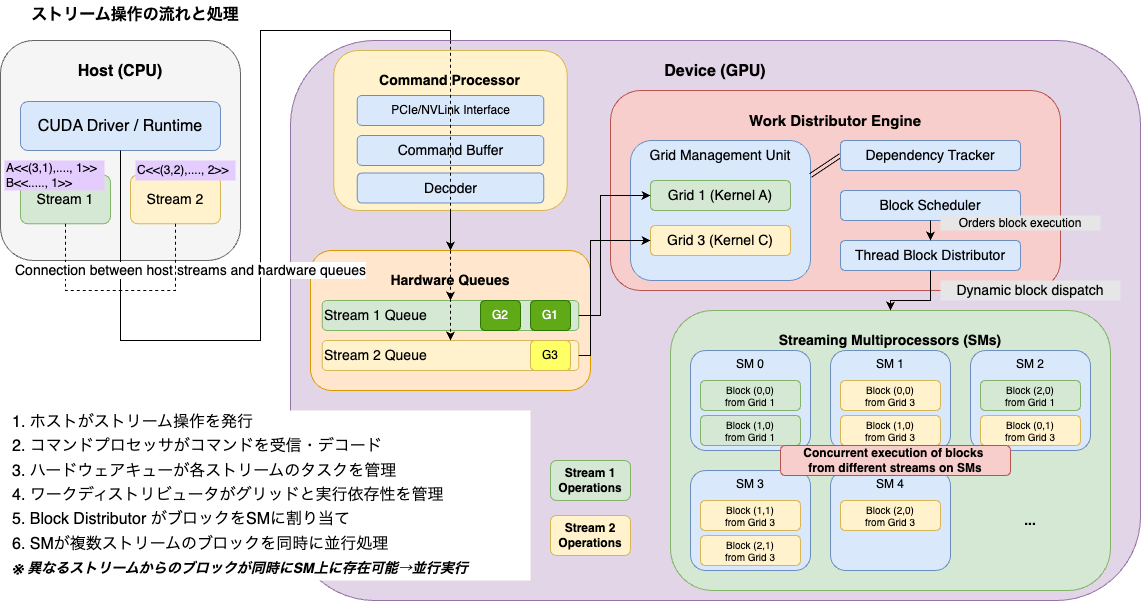
\includegraphics[scale=0.32]{img/grid-advanced_ver2.png}
  \end{figure}
\end{frame}
%%%%%
\begin{frame}[fragile]{Interlude: template to use multiple Streams}
  \begin{lstlisting}[language=CUDA]
cudaStream_t sCompute, sCopy;
cudaStreamCreate(&sCompute);
cudaStreamCreate(&sCopy);

// 1) 非同期コピー(H→D)を stream sCopy
cudaMemcpyAsync(d_in,  h_in,  bytes, cudaMemcpyHostToDevice, sCopy);

// 2) カーネルを stream sCompute
myKernel<<<grid, block, 0, sCompute>>>(d_in, d_out);  // 0: sharedMem ID, 

// 3) 非同期コピー(D→H)を stream sCopy
cudaMemcpyAsync(h_out, d_out, bytes, cudaMemcpyDeviceToHost, sCopy);

// 4) 任意の同期点
cudaEvent_t done;  cudaEventCreate(&done);
cudaEventRecord(done, sCopy);           // sCopy 完了後に立つ
cudaStreamWaitEvent(sCompute, done, 0); // sCompute は done まで待つ
\end{lstlisting}
\end{frame}
%%%%%
\begin{frame}{(+) Using multiple Devices}

\end{frame}
%%%%%%%%%
\subsection{Memory Hierarchy in CUDA}
%%%%%
\begin{frame}{Memory hierarchy of NVIDIA GPU}
 % global memory, shared memory, cache etc. Clarify which programmers can explicitly use

\end{frame}
%%%%%
\begin{frame}{Tiling: effective use of shared memory}

\end{frame}
%%%%%%%%
\subsection{Resolving race condition on CUDA}
%%%%%
\begin{frame}{To avoid race conditions: effective use of parameters}

\end{frame}
%%%%%
\begin{frame}{To avoid race conditions: barrier synchronization}

\end{frame}
%%%%%
\begin{frame}{To avoid race conditions: Cooperative groups}

\end{frame}
%%%%%%%%
\begin{frame}{(Reluctantly) resolve race conditions: Atomic accumulations}

\end{frame}
%%%%%%%%%%%%%%%%%%%%%%%%%%%%%%%
%\section{Optimize CUDA program}
%% 目次
%\begin{frame}{Contents}
%    \begin{enumerate}[<+->]   % <+-> で 1 行ずつ出現
%    \item \textcolor{gray}{What is CUDA?: Introduction}
%    \item \textcolor{gray}{A CUDA program for beginners}
%    \item \textcolor{gray}{How CUDA works}
%    \item Optimize CUDA program
%    \begin{enumerate}
%      \item How to measure performance?
%      \item Choosing a good block size for performance
%      \item Using shared memory effectively
%      \item Example: matrix multiplication
%    \end{enumerate}
%    \item \textcolor{gray}{Practice Problems}
%  \end{enumerate}
%\end{frame}
%%%%%%%%%
%\begin{frame}{How to measure performance: }
%
%\end{frame}
%%%%%%
%\begin{frame}{How to measure performance: }
%
%\end{frame}
%%%%%%%%%
%\begin{frame}{Matmul program (naive implementation)}
%
%\end{frame}
%%%%%%%%%
%\begin{frame}{Choosing a good block size, thread dim}
%
%\end{frame}
%%%%%%%%
%\begin{frame}{Using shared memory, cache effectively}
%
%\end{frame}
%%%%%%%%
%\begin{frame}{Optimized matmul program}
%
%\end{frame}
%%%%%%%%%%%%%%%%%%%%%%%%%%%%%%%
% 目次
\begin{frame}{Contents}
 \begin{enumerate}   % <+-> で 1 行ずつ出現
   \item \textcolor{gray}{What is CUDA?: Introduction}
   \item \textcolor{gray}{A CUDA program for beginners}
   \item \textcolor{gray}{How CUDA works}
   \item \textcolor{gray}{Optimize CUDA program}
   \item Practice Problems
   \begin{enumerate}
     \item k-NN for vector Database
     \item SW's local alignment; DP acceleration with GPU
   \end{enumerate}
 \end{enumerate}
\end{frame}
%%%%%%%%
%\begin{frame}{Problem \#1: k-NN for vector Database}
%
%\end{frame}
%%%%%%
%\begin{frame}{Hint: How to launch kernel across multiple GPUs}
%
%\end{frame}
%%%%%%%%%
%\begin{frame}{Problem \#2: local alignment of DNA arrays}
%
%\end{frame}
%%%%%
\begin{frame}{Smith Water 's DP}

\end{frame}
%%%%%%%%
\begin{frame}{Further problems ...}
 % list of mundane problems

\end{frame}
%%%%%%%%%%%%%%%%%%%%%%%%%%%%%%%
%\begin{frame}{References}
%  \begin{enumerate}
%    \item \url{https://docs.nvidia.com/cuda/parallel-thread-execution/#}
%    \item \url{https://docs.nvidia.com/cuda/cuda-c-programming-guide/index.html#}
%    \item \url{https://docs.nvidia.com/cuda/cuda-runtime-api/index.html}
%    \item \url{https://www.nas.nasa.gov/hecc/support/kb/basics-on-nvidia-gpu-hardware-architecture_704.html}
%    \item %\url{https://developer.nvidia.com/blog/unified-memory-cuda-beginners/}
%    \item %\url{https://www.nvidia.com/content/pdf/fermi_white_papers/p.glaskowsky_nvidia's_fermi-the_first_complete_gpu_architecture.pdf}
%    \item %\url{https://developer.nvidia.com/ja-jp/blog/nvidia-hopper-architecture-in-depth/}
%  \end{enumerate}
%\end{frame}
%%%%%%%%%%%%%%%%%%%%%%%%%%%%%%
\end{document}
